\begin{figure*}[ht]
  \centering
    \begin{subfigure}[b]{0.49\textwidth}
        \centering
        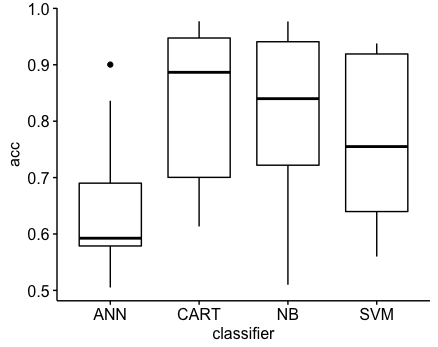
\includegraphics[width=\textwidth]{Rplots/boxplot_classifiers.png}
        \caption[]%
        {{\small}}
        \label{fig:box_classifers}
    \end{subfigure}
  \hfill
    \begin{subfigure}[b]{0.49\textwidth}
        \centering
        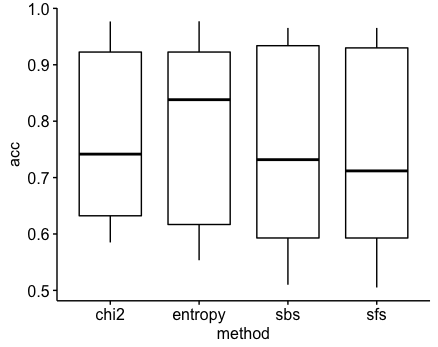
\includegraphics[width=\textwidth]{Rplots/boxplot_methods.png}
        \caption[]%
        {{\small}}
        \label{fig:box_methods}
    \end{subfigure}
  \caption[]
  {\small Variation in accuracy in respect to (a) classifiers and (b) FS-methods. Vertical axis represents accuracy. The horizontal bar in each box represents the mean accuracy. The box represents the range where 50\% of the measurements was found. The vertical lines connected to the boxes includes represents the remaining 25\% on each side. Dots represents outliers.}
  \label{fig:box_plots}
\end{figure*}
